
% specify document type: 
% types of document classes: article, IEEEtran, proc, report, book, slides, memoir, letter, beamer
\documentclass[11pt]{article}

% packages

% usual packages used for psets
\usepackage[margin=1in]{geometry} 
\usepackage{amsmath,amsthm,amssymb}
\usepackage{enumerate}

% image packages
\usepackage{graphicx}
\usepackage{float}
\graphicspath{ {images/} }

% bib packages
\usepackage[
	backend=biber,
	style=numeric,
	% stylename: numeric, alphabetic, authoryear, authortitle verbose etc.
	% https://www.sharelatex.com/learn/Biblatex_bibliography_styles
	sorting=ynt]{biblatex}
% bib resource name
\usepackage[utf8]{inputenc}
\addbibresource{sample.bib}


% you can make new commands!
\newtheorem{theorem}{Theorem}
\newtheorem{corollary}[theorem]{Corollary}
\newtheorem{lemma}[theorem]{Lemma}
\newtheorem{observation}[theorem]{Observation}
\newtheorem{example}[theorem]{Example}
\newtheorem{definition}[theorem]{Definition}
\newtheorem{claim}[theorem]{Claim}
\newtheorem{fact}[theorem]{Fact}
\newtheorem{assumption}[theorem]{Assumption}

% define your own macros!

\newcommand{\code}[1]{\texttt{#1}}
\newcommand{\R}{{\mathbb R}} 
\renewcommand{\vector}[1]{(x_1,x_2,\ldots,x_{#1})} %overriding existing macros
\newcommand{\avector}[2]{(#1_1,#1_2,\ldots,#1_{#2})}
\newcommand{\aDEFvector}[2][a]{(#1_1,#1_2,\ldots,#1_{#2})}


% start document
\begin{document}

% doesn't really matter where this goes, as long as it's before maketitle
\title{Introduction to Latex \thanks{Special thanks to Lesley, Alan, Will}}
\author{Flora Park}

% creates a title for you
\maketitle

\section*{Basic Commands for Latex}
	\subsection*{How to compile a .tex file}
	Here are some general commands we need to know:
	\begin{itemize}
		\item \code{pdflatex file.tex}: to create pdf with latex file into a pdf
		\item \code{open file.pdf}: open the pdf file
	\end{itemize}
	\subsection*{How to write in Latex?}
	Writing in Latex is pretty similar to any other document editing software, e.g. Microsoft Word. The slight difference is that it allows you to switch back and forth in math mode, which is convenient if you are writing text files that have more equations, etc. in them.

	\subsection*{Some handy commands/ resources}
	\begin{itemize}
		\item \code{\textbackslash begin\{itemize\},\textbackslash end\{itemize\}}, each item denoted \code{\textbackslash item}
		\item \code{\textbackslash section\{\}}, unnumbered \code{\textbackslash section*\{\}}, \code{\textbackslash subsection\{\}}
		\item Consider the following vectors with entries in $\R$:\\ $\mathbf
x=\vector{6}$, $\mathbf u=\avector{u}{7}$, $\mathbf a=\aDEFvector{8}$,
$\mathbf w=\aDEFvector[w]{n+1}$.
	\end{itemize}

	\begin{itemize}
		\item Detextify: \textbf{detexify.kirelabs.org/classify.html}
		\item Sharelatex: https://www.sharelatex.com/
		\item TeXShop
	\end{itemize}

\section*{Defining your own macros}

\section*{Numbering your theorems, equations, etc.}
	\begin{theorem} first theorem \end{theorem}
	\begin{theorem} second theorem \end{theorem}
	\begin{theorem} third theorem \end{theorem}
	\begin{claim} first claim \end{claim}
	\setcounter{theorem}{0}
	\begin{claim} second claim \end{claim}
	\begin{equation}
		\label{other} x_1 + \ldots + x_n = \dfrac{10^n}{n} \cdot \sqrt{x_{n} + x_{n+1}}
	\end{equation}
	\begin{equation}
		\label{power} \sum_{i=0}^{\infty} a_i x^i
	\end{equation}
	
	The equation \ref{power} is a typical power series.

\section*{Expanding on mathematical equations, proof of work}
\begin{theorem} $\mid V_i(s, u, r_i+1) - V_i(s, u, r_i) \mid \leq 2b$
\end{theorem}

\begin{proof}

Let's denote $s_j$ and $u_j$ as $s_j$ = $ s + jl_{i+1}$ and $u_j$ = $ u + jl_{i+1} + r_i$.
\[
	V_i(s, u, r_i+1) - V_i(s, u, r_i) \newline
	= \sum_{j=0}^{j=b-1} \{ \mathcal{E}_{i+1}(s_j, u_j+1) + \mid r_i +1 \mid - \mathcal{E}_{i+1}(s_j, u_j) - \mid r_i \mid \}
\]
By change of variables $ r_{{i+1}, j} + 1 = r'$:
\begin{flalign*}
    \mathcal{E}_{i+1}(s_j, u_j + 1) &= \min ( T_{i+1}(s_j, u_j+1+r_{{i+1}, j}) + \mid r_{{i+1}, j} \mid ) \\
    &= \min ( T_{i+1}(s_j, u_j + r')  + \mid r' - 1 \mid ) \\ 
    & \leq \min (T_{i+1}(s_j, u_j + r')  + \mid r' \mid ) + 1\\ 
    &=  \mathcal{E}_{i+1}(s_j, u_j ) + 1
\end{flalign*}

Similarly,
\begin{flalign*}
    \mathcal{E}_{i+1}(s_j, u_j + 1) &= \min ( T_{i+1}(s_j, u_j+1+r_{{i+1}, j}) + \mid r_{{i+1}, j} \mid ) \\
    &= \min ( T_{i+1}(s_j, u_j + r')  + \mid r' - 1 \mid ) \\ 
    &\geq \min (T_{i+1}(s_j, u_j + r')  + \mid r' \mid ) - 1\\ 
    &=  \mathcal{E}_{i+1}(s_j, u_j ) - 1
\end{flalign*}

$\therefore$ for every $j$ value, $ \mathcal{E}_{i+1}(s_j, u_j) -1 \leq \mathcal{E}_{i+1}(s_j, u_j +1) \leq \mathcal{E}_{i+1}(s_j, u_j) + 1 $
\begin{flalign*}
\mid V_i(s, u, r_i+1) - V_i(s, u, r_i) \mid &= \sum_{j=0}^{j=b-1} \{ \mathcal{E}_{i+1}(s_j, u_j+1) + \mid r_i +1 \mid - \mathcal{E}_{i+1}(s_j, u_j) - \mid r_i \mid \} \\
	&\leq \sum_{j=0}^{j=b-1} \{ \mathcal{E}_{i+1}(s_j, u_j+1) - \mathcal{E}_{i+1}(s_j, u_j) \} + b \textnormal{ } \\
	&\leq \textnormal{ }b+ b \textnormal{ }\\
	&= \textnormal{ }2b
\end{flalign*}
\end{proof}

\section*{Adding Figures, Tables, etc.}

\subsection*{Inserting a picture with captions}
%shorthand version 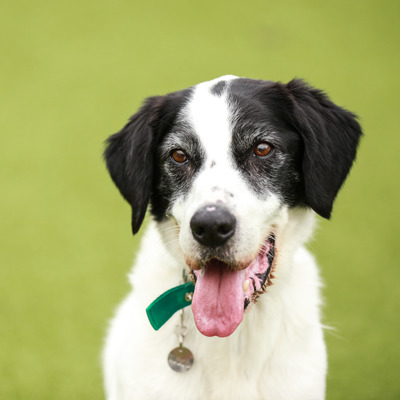
\includegraphics[scale=1]{dog1}
\begin{figure}[H]
	\begin{center}
	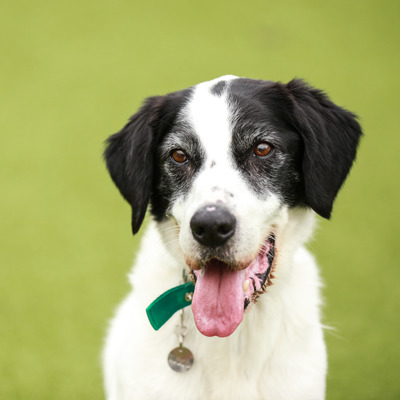
\includegraphics[scale=0.5]{dog1}
	\caption{This is a doggo}
	\end{center}
\end{figure}

\begin{figure}[H]
	\begin{center}
	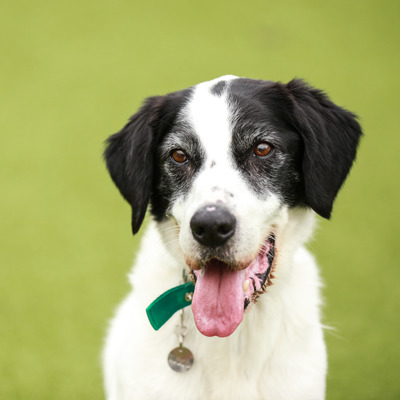
\includegraphics[scale=0.5]{dog1}
	\caption{This is a doggo}
	\end{center}
\end{figure}

%h	Place the float here, i.e., approximately at the same point it occurs in the source text (however, not exactly at the spot)
%t	Position at the top of the page.
%b	Position at the bottom of the page.
%p	Put on a special page for floats only.
%!	Override internal parameters LaTeX uses for determining "good" float positions.
%H	Places the float at precisely the location in the LATEX code. Requires the float package. This is somewhat equivalent to h!.


\subsection*{Inserting a table}

\begin{center}
\begin{tabular}{ |c|c|||c|c| } 
 \hline
 \hline
 \hline
 cell1 & cell2 & cell3 & cell0 \\ 
 cell4 & cell5 & cell6 \\ 
 cell7 & cell8 & cell9 \\ 
 \hline
\end{tabular}
\end{center}

\section*{How to reference your bibliography}




Let's say that we want to cite \cite{knuthwebsite}. We also want to make sure we cite \cite{Vickrey1961} and \cite{Golumbic2004}. Also \cite{einstein}, \cite{dirac}.



%- Small gotchas (like using backticks and double apostrophes for double quotes)
%- Defining your own macros
%- References (e.g. how to reference an equation? Or another section?)
%- Common packages / a latex template
%- Maybe some cute trivia? Like TeX's versioned at `3.1415926`, with `3.14159265` coming up ne
% creating a table
% linking images
% how to do math mode and how to reference them correctly
% 
\printbibliography

% some cool sortings you can do with bibliographies

\printbibliography[type=article,title={Articles only}]
\printbibliography[type=book,title={Books only}]
 
\printbibliography[keyword={physics},title={Physics-related only}]
\printbibliography[keyword={latex},title={\LaTeX-related only}]


% general commands on terminal

% biber file : might be needed for bibilography

\end{document}